\section{Selective Layer Aggregation}

The selective layer aggregation mechanism is the key innovation that enables our framework to balance universal chess knowledge with playstyle-specific strategies. Rather than applying uniform federated averaging across all network parameters, we partition the network into functional layer groups and selectively choose which groups to aggregate across clusters. This section details the layer sharing strategy, the algorithmic implementation, the knowledge transfer mechanisms, and the expected convergence properties.

Figure~\ref{fig:layer-sharing} illustrates how different layer groups are treated during inter-cluster aggregation, with shared layers receiving cross-cluster knowledge transfer while cluster-specific layers remain isolated. Figure~\ref{fig:sharing-configs} presents the experimental configurations we evaluate, showing different hypotheses about which layers benefit from sharing..

\begin{figure}[htbp]
\centering
\begin{tikzpicture}[
    scale=1,
    transform shape,
    node distance=0.25cm,
    layer/.style={rectangle, draw=black, minimum width=3.5cm, minimum height=0.6cm, font=\scriptsize},
    shared/.style={fill=green!30},
    tactical/.style={fill=red!20},
    positional/.style={fill=blue!20},
    arrow/.style={->, >=stealth, thick}
]

% Tactical cluster (left)
\node[font=\small\bfseries] at (-2.5, 0) {Tactical Cluster};
\node[layer, tactical, below=0.3cm] (t-value) at (-2.5, -0.3) {Value Head};
\node[layer, tactical, below=of t-value] (t-policy) {Policy Head};
\node[layer, tactical, below=of t-policy] (t-late) {Late Blocks (14-19)};
\node[layer, tactical, below=of t-late] (t-middle) {Middle Blocks (7-13)};
\node[layer, shared, below=of t-middle] (t-early) {Early Blocks (1-6)};
\node[layer, shared, below=of t-early] (t-input) {Input Block};

% Positional cluster (right)
\node[font=\small\bfseries] at (2.5, 0) {Positional Cluster};
\node[layer, positional, below=0.3cm] (p-value) at (2.5, -0.3) {Value Head};
\node[layer, positional, below=of p-value] (p-policy) {Policy Head};
\node[layer, positional, below=of p-policy] (p-late) {Late Blocks (14-19)};
\node[layer, positional, below=of p-late] (p-middle) {Middle Blocks (7-13)};
\node[layer, shared, below=of p-middle] (p-early) {Early Blocks (1-6)};
\node[layer, shared, below=of p-early] (p-input) {Input Block};

% Cross-cluster aggregation arrows for shared layers
\draw[arrow, green!60!black, <->, line width=1.5pt] (t-early.east) -- node[above, font=\tiny] {aggregated} (p-early.west);
\draw[arrow, green!60!black, <->, line width=1.5pt] (t-input.east) -- node[above, font=\tiny] {aggregated} (p-input.west);

% X marks for non-shared layers
\node[font=\Large, red] at (0, -0.9) {\texttimes};
\node[font=\Large, red] at (0, -1.7) {\texttimes};
\node[font=\Large, red] at (0, -2.5) {\texttimes};
\node[font=\Large, red] at (0, -3.3) {\texttimes};

% Legend
\node[draw, fill=white, text width=4cm, font=\scriptsize, below=0.5cm of t-input, xshift=2.5cm] {
\textbf{Legend:}\\
\colorbox{green!30}{\phantom{XX}} Shared across clusters\\
\colorbox{red!20}{\phantom{XX}} Tactical-specific\\
\colorbox{blue!20}{\phantom{XX}} Positional-specific
};

\end{tikzpicture}
\caption{Selective layer sharing visualization showing how different layer groups are treated during inter-cluster aggregation in the baseline configuration (B1). Green layers (input block and early residual blocks) are aggregated across clusters, receiving cross-cluster knowledge transfer. Red and blue layers (middle blocks, late blocks, and output heads) remain cluster-specific, preserving strategic preferences. Arrows indicate cross-cluster aggregation; X marks indicate isolated layers.}
\label{fig:layer-sharing}
\end{figure}

\begin{figure}[htbp]
\centering
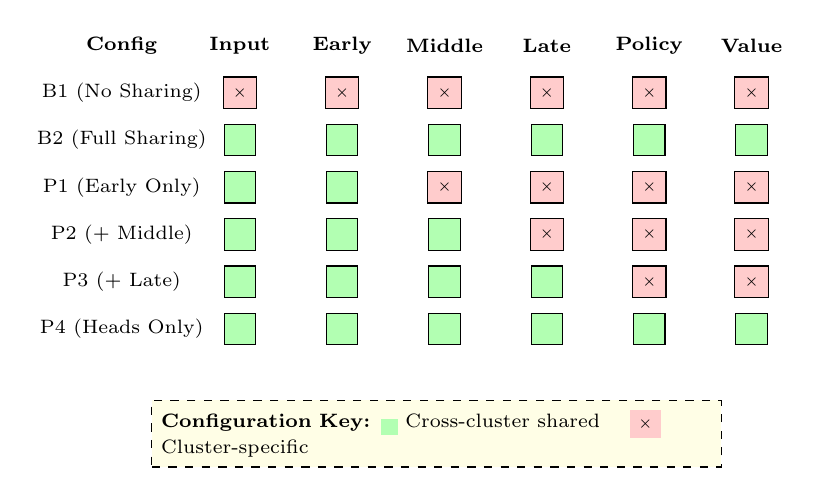
\begin{tikzpicture}[
    scale=1,
    transform shape
]

% Headers
\node[font=\scriptsize\bfseries] at (0, 0) {Config};
\node[font=\scriptsize\bfseries] at (1.5, 0) {Input};
\node[font=\scriptsize\bfseries] at (2.8, 0) {Early};
\node[font=\scriptsize\bfseries] at (4.1, 0) {Middle};
\node[font=\scriptsize\bfseries] at (5.4, 0) {Late};
\node[font=\scriptsize\bfseries] at (6.7, 0) {Policy};
\node[font=\scriptsize\bfseries] at (8, 0) {Value};

% Row labels
\node[font=\scriptsize] at (0, -0.6) {B1 (No Sharing)};
\node[font=\scriptsize] at (0, -1.2) {B2 (Full Sharing)};
\node[font=\scriptsize] at (0, -1.8) {P1 (Early Only)};
\node[font=\scriptsize] at (0, -2.4) {P2 (+ Middle)};
\node[font=\scriptsize] at (0, -3.0) {P3 (+ Late)};
\node[font=\scriptsize] at (0, -3.6) {P4 (Heads Only)};

% B1: No sharing (independent)
\node[draw, fill=red!20, minimum size=0.4cm] at (1.5, -0.6) {\tiny $\times$};
\node[draw, fill=red!20, minimum size=0.4cm] at (2.8, -0.6) {\tiny $\times$};
\node[draw, fill=red!20, minimum size=0.4cm] at (4.1, -0.6) {\tiny $\times$};
\node[draw, fill=red!20, minimum size=0.4cm] at (5.4, -0.6) {\tiny $\times$};
\node[draw, fill=red!20, minimum size=0.4cm] at (6.7, -0.6) {\tiny $\times$};
\node[draw, fill=red!20, minimum size=0.4cm] at (8, -0.6) {\tiny $\times$};

% B2: Full sharing
\node[draw, fill=green!30, minimum size=0.4cm] at (1.5, -1.2) {\tiny $\checkmark$};
\node[draw, fill=green!30, minimum size=0.4cm] at (2.8, -1.2) {\tiny $\checkmark$};
\node[draw, fill=green!30, minimum size=0.4cm] at (4.1, -1.2) {\tiny $\checkmark$};
\node[draw, fill=green!30, minimum size=0.4cm] at (5.4, -1.2) {\tiny $\checkmark$};
\node[draw, fill=green!30, minimum size=0.4cm] at (6.7, -1.2) {\tiny $\checkmark$};
\node[draw, fill=green!30, minimum size=0.4cm] at (8, -1.2) {\tiny $\checkmark$};

% P1: Input + Early shared
\node[draw, fill=green!30, minimum size=0.4cm] at (1.5, -1.8) {\tiny $\checkmark$};
\node[draw, fill=green!30, minimum size=0.4cm] at (2.8, -1.8) {\tiny $\checkmark$};
\node[draw, fill=red!20, minimum size=0.4cm] at (4.1, -1.8) {\tiny $\times$};
\node[draw, fill=red!20, minimum size=0.4cm] at (5.4, -1.8) {\tiny $\times$};
\node[draw, fill=red!20, minimum size=0.4cm] at (6.7, -1.8) {\tiny $\times$};
\node[draw, fill=red!20, minimum size=0.4cm] at (8, -1.8) {\tiny $\times$};

% P2: + Middle
\node[draw, fill=green!30, minimum size=0.4cm] at (1.5, -2.4) {\tiny $\checkmark$};
\node[draw, fill=green!30, minimum size=0.4cm] at (2.8, -2.4) {\tiny $\checkmark$};
\node[draw, fill=green!30, minimum size=0.4cm] at (4.1, -2.4) {\tiny $\checkmark$};
\node[draw, fill=red!20, minimum size=0.4cm] at (5.4, -2.4) {\tiny $\times$};
\node[draw, fill=red!20, minimum size=0.4cm] at (6.7, -2.4) {\tiny $\times$};
\node[draw, fill=red!20, minimum size=0.4cm] at (8, -2.4) {\tiny $\times$};

% P3: + Late
\node[draw, fill=green!30, minimum size=0.4cm] at (1.5, -3.0) {\tiny $\checkmark$};
\node[draw, fill=green!30, minimum size=0.4cm] at (2.8, -3.0) {\tiny $\checkmark$};
\node[draw, fill=green!30, minimum size=0.4cm] at (4.1, -3.0) {\tiny $\checkmark$};
\node[draw, fill=green!30, minimum size=0.4cm] at (5.4, -3.0) {\tiny $\checkmark$};
\node[draw, fill=red!20, minimum size=0.4cm] at (6.7, -3.0) {\tiny $\times$};
\node[draw, fill=red!20, minimum size=0.4cm] at (8, -3.0) {\tiny $\times$};

% P4: Heads only specific
\node[draw, fill=green!30, minimum size=0.4cm] at (1.5, -3.6) {\tiny $\checkmark$};
\node[draw, fill=green!30, minimum size=0.4cm] at (2.8, -3.6) {\tiny $\checkmark$};
\node[draw, fill=green!30, minimum size=0.4cm] at (4.1, -3.6) {\tiny $\checkmark$};
\node[draw, fill=green!30, minimum size=0.4cm] at (5.4, -3.6) {\tiny $\checkmark$};
\node[draw, fill=green!30, minimum size=0.4cm] at (6.7, -3.6) {\tiny $\checkmark$};
\node[draw, fill=green!30, minimum size=0.4cm] at (8, -3.6) {\tiny $\checkmark$};

% Legend
\node[draw, dashed, fill=yellow!10, text width=7cm, font=\scriptsize, below=0.3cm] at (4, -4.2) {
\textbf{Configuration Key:}
\colorbox{green!30}{\tiny $\checkmark$} Cross-cluster shared \quad
\colorbox{red!20}{\tiny $\times$} Cluster-specific
};

\end{tikzpicture}
\caption{Experimental layer sharing configurations tested to evaluate selective aggregation hypotheses. B1 and B2 are baseline configurations with no sharing (independent clusters) and full sharing (standard federated learning) respectively. P1-P4 represent selective sharing configurations that progressively increase the number of shared layer groups to test hypotheses about which layers benefit from cross-cluster aggregation. Green checkmarks indicate shared layers; red X marks indicate cluster-specific layers.}
\label{fig:sharing-configs}
\end{figure}

\subsection{Layer Sharing Strategy}

The layer sharing strategy determines which of the five layer groups (input block, early residual blocks, middle residual blocks, late residual blocks, policy head, value head) undergo cross-cluster aggregation versus remaining cluster-specific. This decision reflects hypotheses about the hierarchical nature of chess knowledge representation in deep neural networks.

We evaluate our selective aggregation approach against two baseline configurations. B1 represents fully independent training with no cross-cluster sharing, serving as a lower bound on knowledge transfer. B2 represents standard federated learning with complete parameter sharing across all layers, serving as an upper bound on knowledge transfer but potentially sacrificing playstyle preservation. Our selective configurations (P1-P4) explore the middle ground between these extremes.

Configuration P1 designates the input block and early residual blocks as shared layers while keeping middle blocks, late blocks, and both output heads cluster-specific. This configuration embodies our primary hypothesis that early layers learn universal low-level patterns applicable to all chess positions regardless of playstyle, such as basic piece relationships, attack and defense patterns, and elementary tactical motifs. These fundamental patterns should benefit from training data across all playstyles, as they represent chess knowledge that transcends strategic preferences.

Middle and late residual blocks are kept cluster-specific because they learn increasingly abstract and strategic representations. Middle blocks that learn tactical patterns may differ between clusters that emphasize aggressive piece activity versus solid defensive structures. Late blocks that integrate strategic evaluation may encode fundamentally different position assessment criteria between tactical and positional clusters. Maintaining separate parameters for these layers allows each cluster to develop specialized strategic understanding appropriate to its playstyle.

The output heads are cluster-specific because they directly encode move selection preferences and position evaluation. The policy head in a tactical cluster should favor sacrifices, attacks, and dynamic imbalances, while the policy head in a positional cluster should favor prophylaxis, structure, and long-term advantages. Similarly, the value head's assessment of position quality depends on strategic criteria that differ between playstyles. Keeping these heads separate ensures that the final predictions reflect cluster-specific strategic judgment.
\subsection{Weight Aggregation Algorithm}

The selective weight aggregation algorithm extends standard federated averaging to operate independently on different layer groups. The algorithm maintains separate aggregation logic for shared and cluster-specific layers, ensuring that cross-cluster knowledge transfer occurs only where desired.

Let $\mathcal{L}_{\text{shared}}$ denote the set of layer groups designated for cross-cluster sharing, and let $\mathcal{L}_{\text{specific}}$ denote the layer groups maintained cluster-specifically. For our baseline configuration, $\mathcal{L}_{\text{shared}} = \{\text{input block}, \text{early residual blocks}\}$ and $\mathcal{L}_{\text{specific}} = \{\text{middle residual blocks}, \text{late residual blocks}, \text{policy head}, \text{value head}\}$.

During inter-cluster aggregation at round $t$, the server receives cluster-specific models $\theta_{\text{tactical}}^{(t)}$ and $\theta_{\text{positional}}^{(t)}$ from the intra-cluster aggregation tier. For each shared layer group $g \in \mathcal{L}_{\text{shared}}$, the server computes the cross-cluster average:

\begin{equation}
\theta_g^{(t+1)} = \frac{n_{\text{tactical}} \theta_{\text{tactical},g}^{(t)} + n_{\text{positional}} \theta_{\text{positional},g}^{(t)}}{n_{\text{tactical}} + n_{\text{positional}}}
\end{equation}

where $n_c$ represents the total training examples processed by cluster $c$ since the last inter-cluster aggregation. This weighted average reflects the relative contributions of each cluster to the shared representation.

For cluster-specific layer groups $g \in \mathcal{L}_{\text{specific}}$, no cross-cluster aggregation occurs. Each cluster's parameters remain unchanged:

\begin{equation}
\theta_{\text{tactical},g}^{(t+1)} = \theta_{\text{tactical},g}^{(t)}, \quad \theta_{\text{positional},g}^{(t+1)} = \theta_{\text{positional},g}^{(t)}
\end{equation}

The server then constructs updated cluster models by combining shared and cluster-specific parameters. For each cluster $c$, the updated model is:

\begin{equation}
\theta_c^{(t+1)} = \bigcup_{g \in \mathcal{L}_{\text{shared}}} \theta_g^{(t+1)} \cup \bigcup_{g \in \mathcal{L}_{\text{specific}}} \theta_{c,g}^{(t+1)}
\end{equation}

This composite model contains cross-cluster averaged parameters for shared layers and cluster-preserved parameters for specific layers. The server distributes these updated models back to their respective clusters, where they replace the cluster-specific models produced by intra-cluster aggregation.
\subsection{Knowledge Transfer Mechanism}

The selective aggregation mechanism enables a specific form of knowledge transfer where universal chess patterns propagate across clusters while strategic preferences remain isolated. This transfer occurs through the shared layer parameters, which act as a common foundation upon which cluster-specific specializations are built.

Shared early layers learn feature representations that apply across all training data, regardless of cluster origin. When a tactical client discovers an effective pattern for detecting knight forks and a positional client learns to recognize weak square complexes, both patterns become encoded in the shared early layer parameters through cross-cluster aggregation. Subsequent training in both clusters can then build upon this expanded pattern library, even though individual clients never directly observe the other cluster's training games.

The knowledge transfer is asymmetric in depth. Low-level patterns in shared layers benefit from the full diversity of training experiences across all clusters. Middle-layer tactical motifs and late-layer strategic concepts remain cluster-specific, allowing each cluster to develop specialized higher-level representations on top of the shared foundation. The policy and value heads, which directly determine move selection and position evaluation, receive no cross-cluster influence and purely reflect cluster-specific strategic preferences.

This hierarchical transfer mechanism aims to capture the intuition that chess knowledge has both universal and style-dependent components. Basic patterns like piece mobility, king safety threats, and material imbalances apply universally and should be learned from diverse data. Strategic concepts like acceptable pawn weaknesses, piece activity versus structure trade-offs, and long-term versus short-term thinking vary with playstyle and should be learned within specialized clusters. The selective aggregation architecture embodies this hierarchical separation.

\subsection{Convergence Properties}

The selective aggregation approach introduces complexity to the convergence analysis compared to standard federated learning. Cluster-specific layers converge to solutions that minimize loss over their cluster's data distribution, while shared layers converge to solutions that minimize loss over the combined distribution of all clusters.

For cluster-specific layer groups, convergence follows standard federated averaging analysis within each cluster. Since these layers never receive cross-cluster updates, each cluster's specific layers converge to optima for their local data distribution. The tactical cluster's late layers and output heads will converge to parameters optimal for tactical positions, while positional cluster layers converge to parameters optimal for positional play.

Shared layer convergence is more complex because these layers receive gradients from diverse data distributions during local training but are synchronized across clusters during inter-cluster aggregation. The shared layers will converge toward parameters that minimize the weighted average of losses across both clusters' data distributions. If tactical and positional training data contain common underlying patterns that benefit from similar low-level representations, the shared layers should converge to parameters that effectively encode these universal patterns. If the distributions are too different and require contradictory low-level features, the shared layers may converge to a compromise solution that serves neither cluster optimally.

The success of selective aggregation depends on the hypothesis that early layers genuinely learn distribution-agnostic patterns. If this hypothesis holds, sharing these layers accelerates convergence by pooling diverse training experiences. If it fails, forcing these layers to be shared may slow convergence or degrade performance. The experimental evaluation examines this hypothesis empirically by comparing selective aggregation against fully independent and fully shared baselines.

